\documentclass{article}
\usepackage{amssymb}
\usepackage{graphicx}

\title{Brief justification to modeling CPU/GPU behaviour}
\author{Álvaro Rodríguez Gallardo}
\date{\today}

\begin{document}

\maketitle

\section{Introduction}

Firstly, we have a problem in which we should use a MultObjective Evolutionary Algorithm (MOEA). In this first approach, execution time and energy consumption are parameters that should be minimised. Because of that, both objective functions must be defined.

In this document, it is going to be justified why \(\frac{1}{{x^p}}\) is a good option to modelise behaviour of CPU or GPU cores (even other hardware components behaviour could be represented by this way).

\section{Mathematical Aspects}

Let \(\forall p \in \mathbb{R^+}\) the real numbers succession 
\[
\frac{1}{{x^p}}
\]

where \(x\) is a positive real number (in next sections it is related with quantity of cores).

Later number \(p\) will tell if function is asociated with a hardware component, and it should be known which is its behaviour: if we set a high number of cores in CPU or GPU, for example, execution time should converges to zero, and the previous function fulfill that.

However, GPU reduces execution time, so number \(p\) discriminates which technology is being used. Because of that, let \(p\), \(q\) positive real numbers, and some properties should be studied.

\subsection{Asymptotic behaviour}

It is true that
\[
\lim_{{x \to \infty}} \frac{1}{{x^p}}=\lim_{{x \to \infty}} \frac{1}{{x^q}}=0
\]

\[
\lim_{{x \to 0}} \frac{1}{{x^p}}=\lim_{{x \to 0}} \frac{1}{{x^q}}=\infty
\]

so this properties must be taken into account when other ones have been studied.

\subsection{Cut Points}

We suppose \(p > q\). Then \(\frac{1}{{x^p}}=\frac{1}{x^q}\) \(\Leftrightarrow\) \({x^p}={x^q}\) \(\Leftrightarrow\) \({x^p}-{x^q}=0\) \(\Leftrightarrow\) \({x^q}({x^{p-q}}-1)=0\). As \(x>0\), we have 
\[
{x^{p-q}}-1=0 \Leftrightarrow {x^{p-q}}=1
\]

If \({p-q} \in \mathbb{N}\) then we have \(p-q\) solutions because of Fundamental Theorem of Algebra. In other case, with some transformations we get the same case: one of cut points is 1. Rest of them are complex or negative numbers, so in our future problem, there is only one cut point in x=1.

\subsection{Monotony}

First of all let two values, \(x=\frac{1}{2}\) and \(x=3\)
\[
	\frac{1}{\frac{1}{2}^p}={2^p} > \frac{1}{3^p}
\]

Besides, we have
\[
	\frac{d}{dx}\left[ \frac{1}{{x^p}} \right] = \frac{d}{dx}\left[x^{-p} \right] = -p \cdot x^{-p-1} < 0 \textbf{ } \forall x>0
\]

so there are not relative extremes, and function decreases.

\subsection{Conclusions}

With previous information, if \(p>q\) and if \(x=\frac{1}{2}\), \(x=3\) then \(\frac{1}{\frac{1}{2}^p}={2^p} > \frac{1}{\frac{1}{2}^q}={2^q}\), \(\frac{1}{3^p} < \frac{1}{3^q}\), so we can confirm the next

\[
	\frac{1}{{x^p}} > \frac{1}{{x^q}} \textbf{ } if \textbf{ } 0<x<1
\]

\[
	\frac{1}{{x^p}} \leq \frac{1}{{x^q}} \textbf{ } if \textbf{ } x \geq 1
\]

\section{Graphics}

In this section it is going to be shown graphically the behaviour mentioned above. I use Jupyter Notebook with Python.

For some values, I plot some graphics (in some cases p value, which is not the same p value in Statistic, is higher than q value, I do that because I want to show that in the last section I said p\(>\)q, but it does not matter).

\begin{verbatim}
import matplotlib.pyplot as plt
import numpy as np

# Arrays p_array y q_array
p_array = [1, 2, 3, 4]
q_array = [4, 3, 2, 1]

# Valores de x para las funciones
x_values = np.linspace(0.1, 5, 1000)

# Crear una matriz de subgráficos
fig, axs = plt.subplots(len(p_array), len(q_array), figsize=(15, 10), sharex=True, sharey=True)

for i, p_value in enumerate(p_array):
    for j, q_value in enumerate(q_array):
        # Calcular las funciones 1/x^p y 1/x^q
        y_p = 1 / np.power(x_values, p_value)
        y_q = 1 / np.power(x_values, q_value)
        
        # Graficar las funciones en el subgráfico correspondiente
        axs[i, j].plot(x_values, y_p, color='red', label=f'p_value={p_value}')
        axs[i, j].plot(x_values, y_q, color='blue', label=f'q_value={q_value}')
        
        # Establecer límites de ejes personalizados
        axs[i, j].set_xlim(0, 5)
        axs[i, j].set_ylim(0, 2)
        
        # Agregar etiquetas y leyenda
        axs[i, j].set_title(f'p_value={p_value}, q_value={q_value}')
        axs[i, j].legend()

plt.tight_layout()
plt.show()
\end{verbatim}

Results are

\begin{figure}[h]
  \centering
  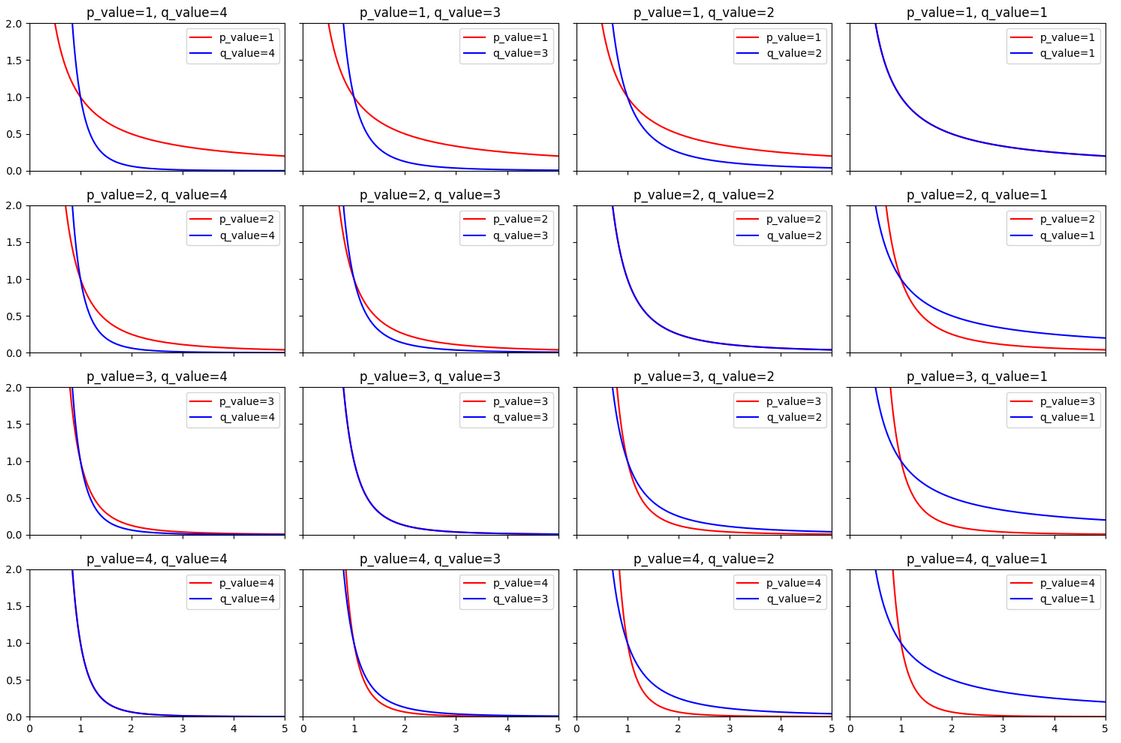
\includegraphics[width=1.3\textwidth]{graficas.png}
  \caption{Graphics in which both functions behaviour is shown}
  \label{fig:etiqueta}
\end{figure}

\end{document}
